\graphicspath{{Images/}}

\section{Ejercicio 2}

\subsection{Consigna}
Para un dado número de procesadores $(n)$ realizar una matriz de transferencia a los fines de detectar posibles heterogeneidades en la velocidad de transferencia de datos entre los procesadores. Analizar la matriz obtenida.

\subsection{Resolución}

\subsubsection{Implementación con MPI}

\lstinputlisting[language=C++]{codigos/main2.cpp}


\subsubsection{Ejecución en cluster}
Tras haber llevado a cabo la implementación del código, lo pase al cluster y lo compile. Habiéndolo compilado pude observar que tenía 4 nodos disponibles para ejecutarlo. Por sugerencia del profesor decidí correrlo de dos maneras:
\begin{enumerate}
  \item Con los 4 nodos y una tarea por nodo.
  \item Con 4 nodos y dos tareas por nodo.
\end{enumerate}

\textbf{Caso 1}

Para correr el primer caso definí el script de SLURM de la siguiente manera:
\begin{figure}[H]
    \centering
    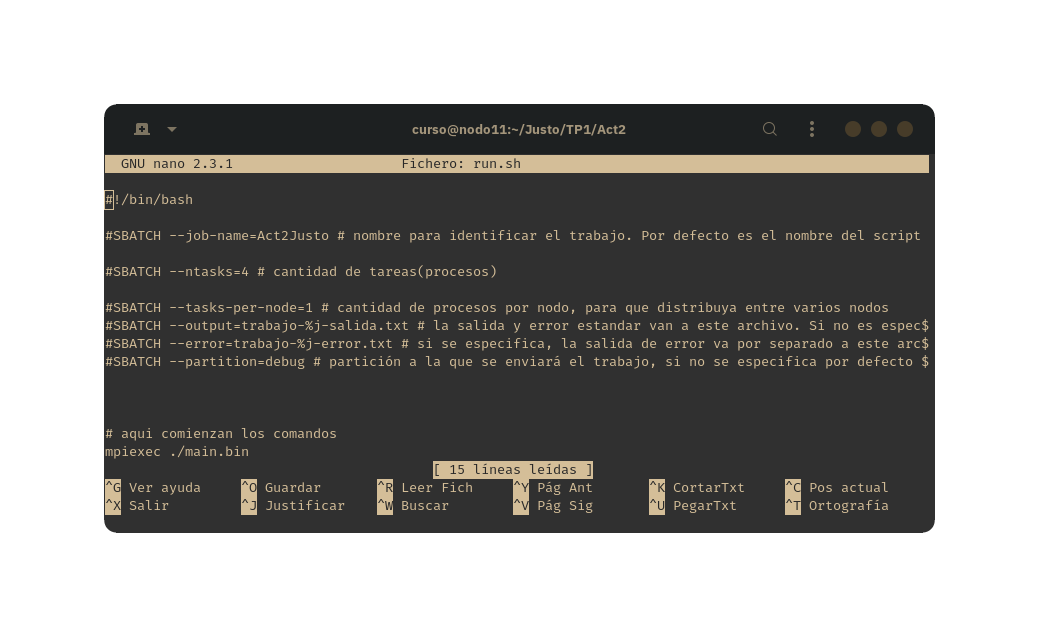
\includegraphics[width=0.80\textwidth]{Images/ej2/scriptcaso1.png}
    \caption{Script para el caso 1}
    \label{fig:scriptcaso1}
\end{figure}

\textbf{Caso 2}
En él el script fue definido de la siguiente manera:
\begin{figure}[H]
    \centering
    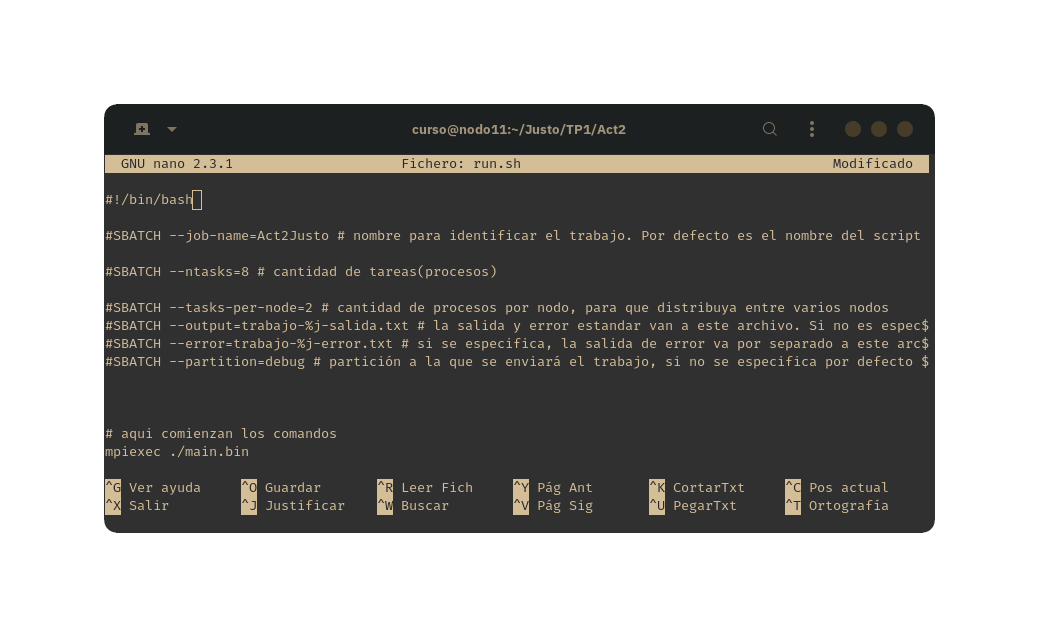
\includegraphics[width=0.80\textwidth]{Images/ej2/scriptcaso2.png}
    \caption{Script para el caso 2}
    \label{fig:scriptcaso2}
\end{figure}

Luego, corrí de igual manera que en el ejercicio 1 (\ref{cap:ej1}) y obtuve las salidas de ambos en mi computadora.


\subsubsection{Análisis}

Teniendo ambos archivos hice un procesamiento de los datos en Python siguiendo la metodología del ejercicio 1 (carga, cálculo del promedio, etc).

Habiendo obtenido un DataFrame para cada caso realicé ciertos cálculos estadísticos, que se ven reflejados en las siguientes tablas: 
\begin{table}[H]
\begin{center}
    \begin{tabular}{| c | c | c | c | }
    \hline
    \multicolumn{2}{|c|}{4 nodos, 1 tarea por nodo} \\ \hline
    Promedio & 0.032750 \\ 
    Desvío & 0.003092 \\ \hline
    \end{tabular}
    \caption{Estadísticos para el caso 1}
    \label{tab:caso1}
\end{center}
\end{table}

\begin{table}[H]
\begin{center}
    \begin{tabular}{| c | c | c | c | }
    \hline
    \multicolumn{2}{|c|}{4 nodos, 2 tareas por nodo} \\ \hline
    Promedio & 0.006535 \\ 
    Desvío & 0.001886 \\ \hline
    \end{tabular}
    \caption{Estadísticos para el caso 2}
    \label{tab:caso2}
\end{center}
\end{table}

Como era de esperarse, el tiempo medio para el caso que tiene más de una tarea por nodo es menor. Esto se debe a que la comunidad entre procesos del mismo nodo es más rápida. 

Luego, realicé mapas de calor para ambos casos de forma que pudiese visualizar gráficamente las diferencias en la latencia.

\textbf{Caso 1}
\begin{figure}[H]
    \centering
    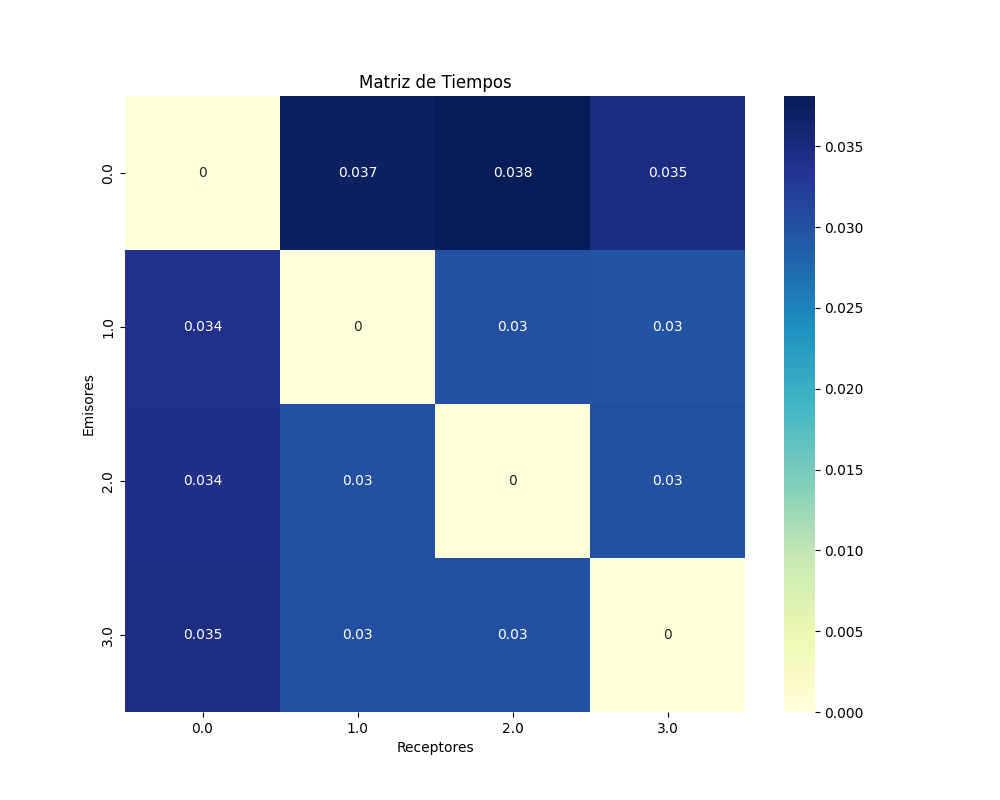
\includegraphics[width=0.80\textwidth]{Images/ej2/matriz1.png}
    \caption{Matriz para el caso 1}
    \label{fig:matrizcaso1}
\end{figure}

Se puede apreciar que cuando tomamos todos nodos distintos, las diferencias son mínimas, y la matriz obtenida es reflejada a través de la diagonal principal.

\textbf{Caso 2}
\begin{figure}[H]
    \centering
    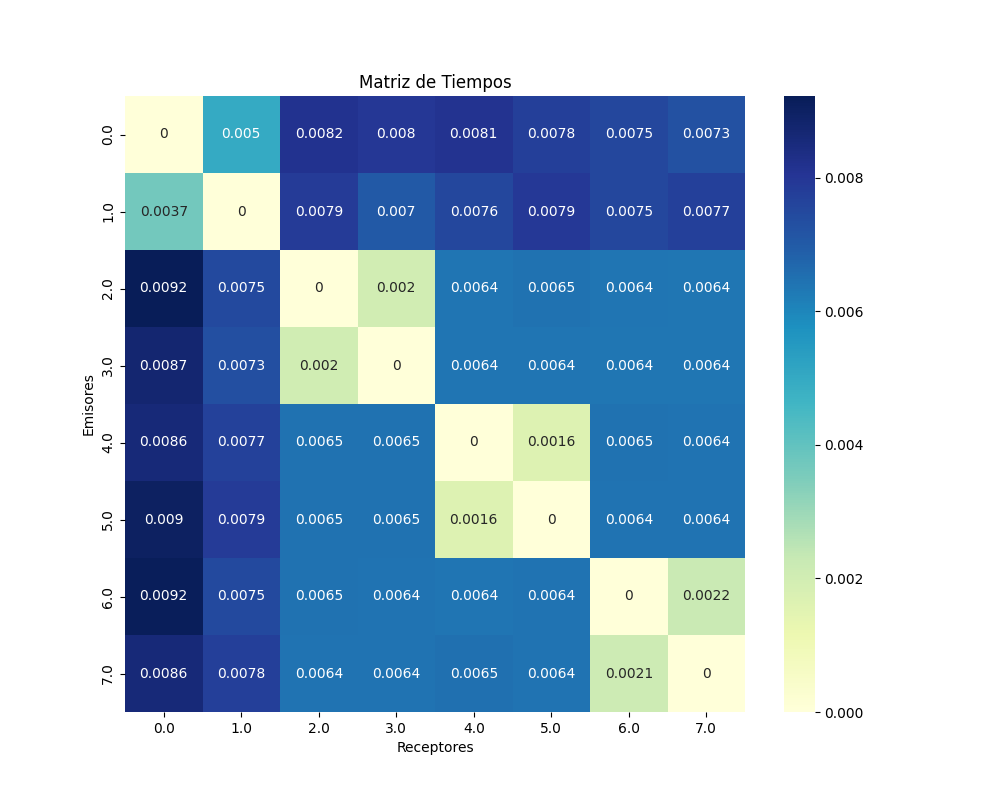
\includegraphics[width=0.80\textwidth]{Images/ej2/matriz2.png}
    \caption{Matriz para el caso 2}
    \label{fig:matrizcaso2}
\end{figure}

En este caso, si vamos tomando de a pares, se pueden ver tiempos muy bajos en comparación con el resto. Esto seguramente se deba a que son procesos que están corriendo en el mismo nodo.